\documentclass[12pt, a4paper]{article}
\usepackage[utf8]{inputenc}
\usepackage[T1]{fontenc}
\usepackage[english]{babel}
\usepackage{geometry}
\geometry{margin=2.5cm}
\usepackage{setspace}
\onehalfspacing
\usepackage{graphicx}
\usepackage{hyperref}
\hypersetup{
    colorlinks=true,
    linkcolor=blue,
    urlcolor=blue,
    citecolor=blue
}
\usepackage{enumitem}
\usepackage{booktabs}
\usepackage{cite}
\usepackage{titlesec}
\usepackage{fancyhdr}
\usepackage{abstract}
\usepackage{microtype}
\usepackage{lmodern}
\usepackage{parskip}

\pagestyle{fancy}
\fancyhf{}
\rhead{\small A\&AD Framework}
\lhead{\small Gasca Buelvas, R.G.}
\cfoot{\thepage}

\begin{document}

% -----------------------------------------------------------------------
% TITLE
% -----------------------------------------------------------------------
\begin{titlepage}
\centering
\vspace*{2cm}
{\LARGE\bfseries The End of Reactive Control: Algorithmic Certainty through Accounting and Audit by Design (A\&AD)\par}
\vspace{1.5cm}
{\large \textbf{Richard G. Gasca Buelvas}\par}
\vspace{0.3cm}
{\normalsize \textit{profesor de c\'atedra del Departamento de Ciencias Contables de la Facultad de Ciencias Econ\'omicas y Administrativas de la Pontificia Universidad Javeriana}\par}
\vspace{0.2cm}
{\normalsize E-mail: \href{mailto:rgasca@javeriana.edu.co}{rgasca@javeriana.edu.co}\par}
\vspace{1cm}
\begin{figure}[h!]
    \centering
    
\includegraphics[width=3cm]{authorship_qr.png}
    
    \vspace{0.2cm}
    {\scriptsize Scan to verify authorship on the Algorand Blockchain\par}
\end{figure}

\begin{quote}
\small\textbf{Disclaimer:} Las opiniones, an\'alisis y conclusiones expresadas en este art\'iculo son de exclusiva responsabilidad del autor y no comprometen ni representan la posici\'on oficial de la Pontificia Universidad Javeriana. / The views, analyses, and conclusions expressed in this paper are solely those of the author and do not compromise, represent, or commit the Pontificia Universidad Javeriana.
\end{quote}
\end{titlepage}

% -----------------------------------------------------------------------
% ABSTRACT
% -----------------------------------------------------------------------
\begin{abstract}
Frameworks for corporate governance and internal control have always tolerated the existence of errors that must be identified after the fact, accepting data desynchronization as an unavoidable transactional friction. The information stored in relational databases must undergo an extensive debugging process to identify the originating event, and this typically occurs long after the fact---when there is no longer any capacity to react. Under this paradigm, financial teams are permanently tasked with reconciling figures across different modules. This process frequently generates multiple spreadsheets outside of core information systems, creating a permanent operational burden that relies heavily on manual, craft-based interventions rather than systemic controls. As a consequence, the visibility available to boards of directors and management is dramatically reduced, both by the timeliness of information and the cost of obtaining it.

To resolve these inefficiencies, this article introduces the Accounting and Audit by Design (A\&AD) framework, designed to industrialize the assurance process into a scalable, repeatable pipeline. The A\&AD model replaces retroactive verification with real-time deterministic assurance at the very moment events occur. By extending the shift-left paradigm to organizational control, A\&AD enforces compliance and fiscal constraints directly at the moment of economic origin---the initial contract or business event. By representing transactions as autonomous and immutable holons within semantic knowledge graphs, leveraging a convergence of global open standards (including ISO/IEC, W3C JSON-LD/SHACL, XBRL, ACTUS, and OMG), internal control ceases to be a manual human intervention to become an intrinsic topological property of the data architecture itself. This approach systematically eliminates subsequent reconciliations, validates regulatory compliance at the exact point of data ingestion, and enables continuous auditing over the entirety of business events.
\end{abstract}

\hrule
\vspace{1em}

% -----------------------------------------------------------------------
% SECTION 1: INTRODUCTION
% -----------------------------------------------------------------------
\section{Introduction \& The Reconciliation Debt}

Since double-entry bookkeeping was invented many centuries ago, accounting has always looked in the rearview mirror. And yes, modern technology and large-scale ERP systems digitized the entire process---but they did not solve the underlying problem. Today, financial records remain flat: static snapshots of economic transactions completely disconnected from the legal contracts and real operations that generated them. It is like having a purchase receipt without knowing why or what the item was bought for. Companies spend fortunes and thousands of hours on reconciliation protocols---not because they do not know how the pieces fit together, but because the reference picture has been obscured: the semantic context that reveals the origin, purpose, and relationships of each transaction has been lost along the way.

This is where the story takes a decisive turn, because we are in the era of artificial intelligence. Large corporations are already allowing autonomous software agents to make decisions: they close supply chain contracts, acquire resources, and execute key business processes. And what happens in our traditional accounting systems when an AI does this? The system records the final number---the expense---but completely erases the context of why the AI made that decision. It becomes a black box that leaves human auditors completely blind.

If we are going to allow AI to manage financial resources at scale, the old approach of statistical sampling becomes not just insufficient---it becomes dangerous. Statistical sampling was a practical necessity when 100\% coverage was humanly impossible. But AI can now process entire populations of transactions. The real risk is that AI applying inference over semantically deficient data does not merely reproduce errors---it magnifies them.

How do we then recover control? How do we rebuild trust in our own systems? The answer requires a radical methodological shift: instead of auditing at month-end, we validate data at the exact second a transaction originates. Building upon the vision of Audit 4.0 and continuous assurance \cite{dai2016}, we propose a Moment~0 Semantic Digital Twin, developed through Design Science Research (DSR). The proposed architecture integrates the Resource-Event-Agent (REA) framework with Semantic Web standards, decoupling the semantic meaning of economic events (using JSON-LD and XBRL GL) from specific software applications. What we fundamentally require is that each business event and its accounting consequences remain semantically coupled---bound together by the logic of their relationship. Storing a numeric value in a spreadsheet cell does neither: it neither identifies the event that caused it, nor describes the obligation or right it generates.

The foundational premise of this work is clear: ERP records are insufficient for automated reporting because they lack semantically coupled business activity---the binding between the originating event, its participants, and its financial consequences. The A\&AD framework presumes this semantic layer can be recovered and, more importantly, captured correctly from the very first instant. A direct and highly desirable consequence of this design is that transactions become self-reconciling: when the semantic context is captured correctly at the point of origin, the need for month-end manual reconciliation disappears entirely. Furthermore, this single source of truth enables a shared reality with multiple points of view: the same transactional event can simultaneously satisfy IFRS, US GAAP, tax, and ESG reporting requirements---each stakeholder querying the same graph from their own perspective, without parallel ledgers or version conflicts. In addition, we introduce the use of hybrid DataBooks \cite{cagle2026} as a standardized transport mechanism. Drawing from the concept of zero-shot learning via ``semantic output codes'' \cite{palatucci2009}, we embed SKOS taxonomies \cite{w3cskos} directly into Large Language Models (LLMs) to act as these strict semantic boundaries. This enables immediate, zero-shot auditing of business events by both human supervisors and autonomous AI oversight agents. The resulting architecture is that of a glass box: all economic activity is traceable, verifiable, and auditable in real time. The rest of this article outlines our theoretical foundations, describes the system architecture of the A\&AD Semantic Twin, and demonstrates an automated, real-time audit of an initial equity distribution.

\hrule
\vspace{1em}

% -----------------------------------------------------------------------
% SECTION 2: RELATED WORK
% -----------------------------------------------------------------------
\section{Related Work \& Theoretical Framework}

The theoretical foundation of the A\&AD architecture lies at the intersection of the Zachman Enterprise Architecture Framework, Tim Berners-Lee's Semantic Web Stack \cite{bernerslee2001}, ontological accounting frameworks, and the audit capabilities of modern generative artificial intelligence. This integration leverages Zachman's structured classification to map organizational questions (What, How, Where, Who, When, Why) directly onto the technical layers of Berners-Lee's Semantic Web Stack---spanning from RDF/OWL representations to rules, cryptographic proofs, and systemic trust layers---aiming to heal the historic division that separates operational business logic from financial ledger records.

\subsection{The REA Paradigm and Graph-Based Digital Twins}

The concept of a Digital Twin traces back to aerospace engineering: originally conceived at NASA---and later formalized by Grieves \cite{grieves2002} at the University of Michigan---it described a virtual replica that mirrors a physical system in real time. The goal was simple but profound: monitor, simulate, and intervene before failures happen in the physical world. When Gartner analysts began describing Digital Twins of Organizations (DTOs), the same logic was transposed to management and operations, positioning DTOs as the connective tissue between day-to-day activity and executive reporting. That is useful. But it is not enough. A financial Semantic Digital Twin cannot stop at mirroring workflows or account balances---it must carry the full semantic weight of the business events that produced those numbers in the first place. That semantic burden is precisely what enables AI Readiness: without it, any AI agent reasoning over financial data is, to put it plainly, reasoning over shadows. This shift---from data-as-output to data-as-context---is what pioneers in enterprise architecture like Dave McComb \cite{mccomb2019} and Cheryl Dunn \cite{dunn2004} have long described under the banner of data-centric architecture: a world where the data model of the enterprise outlasts every software application built on top of it.

To understand how we construct this twin within an accounting framework, one must travel back in time---specifically to 1969. That year, George H.~Sorter proposed something revolutionary: an events approach to accounting theory \cite{sorter1969}. Sorter argued that, instead of relying solely on traditional, highly aggregated financial summaries, systems should record and retrieve detailed data every time an individual economic event occurs. The idea was as simple as it was powerful: give users the granular information they need to make their own decisions.

Years later, in 1997, Shyam Sunder reinforced this vision with his theory of accounting and control, defining the firm as a nexus of contracts \cite{sunder1997}. Think of it this way: a company is nothing more than a sum of agreements among resource providers and individuals who decide to give an entity its origin---our Moment~0---and the accounting system must be there to measure and monitor that these agreements are honored. The A\&AD framework operationalizes this concept by putting Sunder's idea into practice: we represent each contract independently within a semantic knowledge graph. Each contract is a holon---an autonomous node with all its attributes. The result is the ability to track in real time any transaction, event, or condition, as well as the source and use of the corresponding resources.

How do we structure all of this? We build on the theory formalized by William E.~McCarthy (1982): the REA (Resource-Event-Agent) model \cite{mccarthy1982}. McCarthy held that accounting records must reflect the real economic substance of transactions, focusing on the nature of the event, the participants involved, and the resources exchanged. In those days, however, and with the evolution of traditional ERP systems, the REA concept became trapped inside relational tables. Over time, modern researchers have taken the model further, formalizing it into rigorous ontologies such as OntoREA \cite{fischerpauzenberger2017}, capable of representing even the most complex derivative financial portfolios \cite{fischerpauzenberger2018}.

Our approach goes one step further: we directly integrate industry standards such as FIBO \cite{edmc2020} and ACTUS \cite{actus2018} into the transactional graph. And here lies the true topological innovation: we do not route transactions through a relational system (ERP) to later convert them into a graph. We make the contract be born directly in XBRL GL format and, simultaneously, have that instance transmuted into a JSON-LD payload to be injected into the semantic graph. The graph is the original source of truth, and our mission is to keep this ontology hydrated so that it serves as the single source of truth for all the entity's purposes---financial and non-financial alike. Traditional systems can run in parallel or be synchronized in a second phase, but to handle the multidimensional complexity of today's business, the direction is clear: we must evolve from rigid relational database engines toward the absolute flexibility of semantic graphs.

Recognizing that enterprise environments will inevitably rely on fragmented, multi-technology stacks---from legacy SQL relational databases to modern API-driven architectures---this graph-based approach does not attempt to force a single monolithic system. Instead, it provides a universal logical integration layer that maps deterministic business rules across both new and legacy software, bridging the semantic gap that Large Language Models alone cannot solve.

\subsection{Model-Driven Systems, XBRL GL, and Supply Chain Integration}

Historically, a knot has existed between day-to-day business operations and external reporting: two worlds that coexist but do not communicate fluidly. This boundary is precisely what Hoffman's \cite{hoffman2025} Model-Driven Enterprise Architecture attacks. Hoffman proposes something radical but necessary: replacing closed data silos and connecting them through unified, standardized reporting pipelines.

This is where the star of this segment enters: the XBRL Global Ledger (XBRL GL) language. To understand its value, let us make a distinction. While traditional XBRL FR (Financial Reporting) is designed for period-end aggregations, XBRL GL captures and standardizes transactional data at the most granular level possible. Within this standard, the \texttt{accountingPurposeCode} element---a native field defined by XBRL International within the GL taxonomy itself, not an external extension---is crucial: it allows us to classify and tag the purpose of each accounting entry from the exact moment the data is born---whether it is a record for IFRS, US GAAP, or tax purposes. By mapping this tag directly to the semantic graph, we resolve in one stroke the classic problem of maintaining multiple parallel accounting ledgers. The same transactional event can now be queried and filtered dynamically according to the required purpose, ensuring total granularity and eliminating duplication. What is more, the resulting records are capable of self-reconciling.

Implementing XBRL GL as the heart of our data enables total platform-independent interoperability. The audit trail travels intact from its operational genesis---the famous Moment~0---to the regulators, without losing a single drop of semantic meaning along the way. This materializes the foundational vision of the W3C \cite{w3cxbrl} regarding the definitive convergence of XBRL and the Semantic Web.

The A\&AD framework goes further: it extends that power across the entire supply chain, capturing both quantitative financial data and non-financial operational data. By preserving these rich contextual references along the entire information supply chain---from the originating business event directly to the reporting ledger---the Semantic Digital Twin inherently eliminates the traditional, labor-intensive effort of reassembling the audit trail on demand. Thanks to this consolidation in the semantic graph, we can directly generate a statement of financial position and, simultaneously, a corporate sustainability report---the well-known ESG reports---all from the same source of truth, without cumbersome extractions or additional remapping. To govern this multidimensional flow, the framework relies on the Zachman Enterprise Architecture Framework, using its rows and columns to map each operational action directly onto the technical layers of the semantic stack.

Just as XBRL GL and XBRL FR complement each other within the reporting pipeline---the former capturing transactional granularity, the latter aggregating it for disclosure---the Seattle Method proposed by Hoffman \cite{hoffman2025} operates as a natural complement to the A\&AD framework. While Hoffman's approach defines the required disclosure architecture from the top down, A\&AD works bottom-up: it ensures that every economic event is captured with full semantic fidelity at its point of origin, so that the data reaching the disclosure layer is already validated, traceable, and machine-interpretable. The A\&AD pipeline is intentionally designed to be compatible with high-level reporting frameworks---such as XBRL International's Open Information Model (OIM) or the Object Management Group's Standard Business Report Model (SBRM)---where the DataBook serves as the standardized, machine-readable transport container between the transactional origin layer and the disclosure layer.

\subsection{Explainable AI, SKOS Structuring, and DataBooks}

As machine learning models take on increasing responsibilities in financial auditing, the elephant in the room emerges: the risk of artificial intelligence hallucinations. Mitigating this risk is not merely important---it is paramount. We need explainable artificial intelligence.

To achieve this, the framework articulates two complementary tools: the DataBooks of Cagle \cite{cagle2026} and SKOS. DataBooks are hybrid Markdown files containing embedded, machine-readable JSON-LD payloads. What these DataBooks accomplish is the technical magic of the framework: they effectively connect pure narrative texts---legal agreements, incorporation deeds---directly with the structured data in the semantic graphs.

SKOS acts as an auxiliary layer that complements the JSON-LD schema: it organizes concepts, labels, and semantic relationships into a controlled vocabulary that is clearer and more interoperable. This layer is especially valuable when linking the ontology to external standards, such as FIBO or 1EdTech standards for the certification of personnel competencies. With this, we embed W3C SKOS \cite{w3cskos} taxonomies directly into the architecture of Large Language Models (LLMs)---the definitive foundation for explainable AI.

What is the alternative today? Attempting to load supercomplex, multi-volume regulatory rules---such as IFRS or US GAAP---directly into the LLM's temporary context window. This is computationally inefficient and, frankly, drives up error rates. With our architecture, instead, the AI auditing agent leverages the model's pre-existing knowledge of these standardized SKOS structures. The individual DataBook only needs to expose the specific, localized concepts relevant to that particular transaction. This combination allows our auditing agents to evaluate complex graphs with millimetric precision, always bounded by clear ontological limits, thus facilitating continuous, independent monitoring that can be fully trusted.

This architecture instantiates what the AI research community has come to call the \textit{neurosymbolic approach}: the combination of neural language models with formal symbolic reasoning systems. Rather than asking an LLM to infer the rules of IFRS or US GAAP from its training data---a process prone to hallucination and inconsistency---the A\&AD framework anchors the LLM to machine-readable semantic expressions of those standards that already exist in formal ontological form. The symbolic layer constrains; the neural layer communicates. The result is an auditing agent that is both fluent and deterministic.

\hrule
\vspace{1em}

% -----------------------------------------------------------------------
% SECTION 3: ARTIFACT DESIGN
% -----------------------------------------------------------------------
\section{Artifact Design: The A\&AD Semantic Digital Twin}

Consistent with Design Science Research principles \cite{hevner2004}, our primary contribution is the design and implementation of a Semantic Digital Twin. This artifact is built to span what Hoffman \cite{hoffman2025} describes as the operational-regulatory gap, by creating a continuous, verifiable data pipeline from inception to reporting. The architecture comprises a conceptual blueprint and three distinct physical layers: the Conceptual Navigational Matrix, the Operational Graph Engine, the Semantic Transmutation Layer, and the Living Knowledge Wrapper.

\subsection{The Conceptual Blueprint: The A\&AD Navigational Matrix}

The A\&AD Reference Atlas is not a documentation artifact---it is an organizational governance canvas. By fusing Zachman's six interrogatives (What, How, Where, Who, When, Why) with Berners-Lee's Semantic Web Stack, it defines a universal coordinate system for enterprise data governance. Each cell in the matrix represents a governable domain of organizational knowledge: who captures the economic event, how it is validated, what data standard governs it, where it resides, when it is auditable, and why it satisfies a given regulatory requirement. This interactive schema is deployed at \url{https://ai2accountans.github.io/Zachman_Framework_Model/} and serves as the architectural compass that coordinates all engineering layers of the framework.

The current PoC activates a specific set of coordinates---those covered by REA, XBRL GL, FIBO, and ACTUS---establishing financial semantic governance. Crucially, this same canvas extends to any future domain: 1EdTech's CASE ontology for competency and personnel certification governance, TOGAF for IT architecture, or GS1 for physical supply chains. The matrix does not describe data---it maps the jurisdictional reach of the enterprise's semantic intelligence, leaving the canvas activated so that the organization can govern any type of data under the same unifying principles.

\begin{figure}[ht]
\centering

\includegraphics[width=\textwidth]{aad-zachman-atlas.png}
\caption{A\&AD Enterprise Reference Atlas --- Semantic Fusion of Zachman Framework and TBL Semantic Web Stack (Author's Own Work). Interactive version available at \url{https://ai2accountans.github.io/Zachman_Framework_Model/}}
\label{fig:atlas}
\end{figure}

\subsection{The Operational Graph Engine (TerminusDB \& DFRNT)}

At the bottom of the system stack sits TerminusDB---not a conventional relational engine, but something categorically different: a document graph database that operates under closed-world semantics. What does that mean in practice? In financial accounting, a debit entry either exists or it does not. There is no middle ground, no ``probably'' or ``maybe.'' Most graph databases are built on the opposite assumption: if a fact is absent, it is simply unknown. TerminusDB's CWA datalog reasoner flips that logic---any unrecorded fact is treated as false, which is exactly the deterministic guarantee a reliable ledger demands. In building this PoC, we found that this property alone eliminates an entire class of data integrity errors that plague conventional graph implementations. Beyond integrity, the database's immutable append-only architecture unlocks something auditors rarely have access to: genuine bitemporal reasoning. At any moment, we can reconstruct not just what the ledger says now, but what it said---and what was known---at any prior instant. Every JSON-LD document carries its own provenance chain, including who wrote it, when, and under what system state. To navigate and query this graph in production, we rely on the DFRNT semantic data platform, which processes the linked data document graph and exposes it through QOWL (GraphQL over OWL). Our queries home in on the ``Moment~0'' genesis event, pulling not only monetary figures but the full relational lineage of every agent and asset involved.

The choice of TerminusDB over alternative graph databases is deliberate and technically justified on four additional grounds: its built-in OWL reasoner enables automated inference over the ontological relationships without requiring external tooling; its highly flexible schema allows the same data model to represent both operational entities and regulatory taxonomies; its native support for multiple syntaxes---including JSON-LD, Turtle, and SPARQL---ensures zero-friction interoperability with the W3C Semantic Web stack; and its closed-world assumption, as described above, provides the deterministic certainty that financial ledgers demand. DFRNT, as the enterprise interface layer over TerminusDB, further adds collaborative schema versioning, access control, and the QOWL query layer---making it the natural platform for a production-grade financial Digital Twin.

\subsection{The Semantic Transmutation Layer (Altova XMLSpy \& MapForce)}

A critical distinction must be drawn before describing the transmutation process: the A\&AD framework applies not only standard languages and structures---such as XBRL GL as a format or JSON-LD as a syntax---but equally, data standards in the form of classification vocabularies. In accounting, classification is not peripheral---it is the work itself. Whether an item is a current or non-current asset, whether a disbursement is operational or financial---these are foundational claims about what the enterprise can know and report. Standards such as FIBO, ACTUS, and the XBRL GL taxonomy provide precisely these vocabularies: formal, machine-readable assertions about the nature and meaning of economic events. Without them, a semantic graph is merely structure without substance.

Throughout professional practice, a persistent dependence on spreadsheets for building financial reports has been observed. With knowledge of XBRL technology, it is possible to transpose that semantic tagging philosophy to the spreadsheet environment, enabling data enrichment through tags analogous to IFRS classifications---in a highly efficient and cost-effective manner. This practical observation illustrates the central problem: data in CSV, TXT, or Excel format obtained directly from the operational layer of any system typically uses a completely internal vocabulary, lacking the normalized regulatory taxonomy indispensable for auditing and verification. How do we close that gap without falling into the trap of relying on rigidly hardcoded translation rules that would break with any regulatory change?

The answer lies in our architecture, which incorporates the powerful Altova suite as the primary engine of semantic transmutation. The process operates in two major stages:

In the first stage, Altova XMLSpy serves as the schema design environment, where JSON-LD structures are defined and W3C SHACL constraints are applied. This ensures that the core ontology meets all logical consistency criteria before a single real data point is touched.

Once the schema is validated, Altova MapForce enters the field as a format-neutral data mapping engine. From the source JSON payload, MapForce applies the W3C ontologies and the XBRL Global Ledger previously modeled in XMLSpy. The result is pure automation: an automatic transformation of contracts---first into XBRL GL and then into a standardized JSON-LD instance, 100\% compatible with the semantic graph.

And this is where we break with the past. In the traditional XBRL approach, validations and business rules are typically implemented through the \textit{XBRL Formula Linkbase}. In the A\&AD framework, the structural and mathematical validation claims of that linkbase---verifying that debits equal credits, that issuance limits are not exceeded, that required fields are present---are moved directly into the semantic graph and executed via SHACL. This is not a full 1:1 substitution of XBRL Formula: dimensional filtering and period-comparative calculations remain the domain of the XBRL toolchain. What SHACL provides is real-time, graph-native enforcement of the core accounting integrity constraints at the exact moment of data ingestion---before any data is exposed to external review. The result is a shift from post-facto forensic audit to real-time preventive verification: a fundamental change in the temporal position of assurance.

The evolution of this transmutation model---extended toward full supply chain integration under W3C standards---is illustrated in Figure~\ref{fig:chain}.

\begin{figure}[ht]
\centering
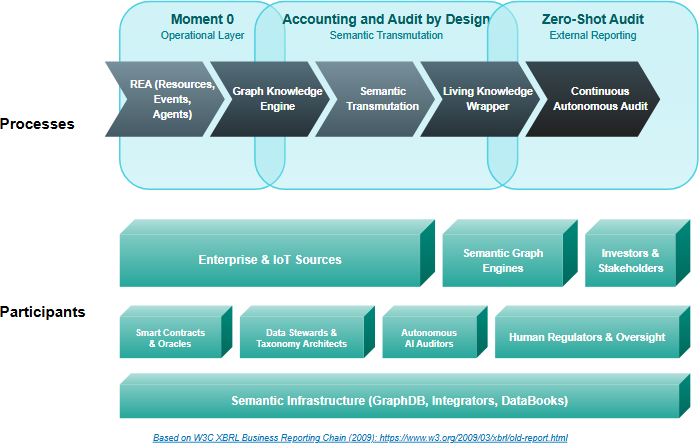
\includegraphics[width=\textwidth]{aad_chain_evolved.png}
\caption{A\&AD Supply Chain Evolution --- W3C Stack (Author's Own Work). Based on W3C XBRL Business Reporting Chain (2009): \url{https://www.w3.org/2009/03/xbrl/old-report.html}}
\label{fig:chain}
\end{figure}

And we are not speculating: this approach has solid industry precedents, as documented by the Maryland Association of CPAs (MACPA) case study, which demonstrated as early as 2010 the absolute viability of using XMLSpy and MapForce to convert heterogeneous accounting ledger databases into perfectly standardized XBRL GL structures \cite{altova2010}.

\subsection{The Living Knowledge Wrapper (DataBooks)}

The final phase of the A\&AD data pipeline handles the interaction between human users and automated systems. The structured JSON-LD output is packaged into a ``DataBook''---a hybrid Markdown document. The DataBook combines a human-readable narrative (such as a corporate charter or partnership agreement) with hidden, machine-readable JSON-LD data segments. This document serves as a self-contained, unchangeable ``holon.'' Human supervisors can review the business context in plain text, while autonomous AI agents can parse the embedded graph data using pre-trained SKOS taxonomies. This decoupled design provides high certainty without requiring the AI to process raw, unstructured language, completing the ``Shift-Left'' audit process.

\hrule
\vspace{1em}

% -----------------------------------------------------------------------
% SECTION 4: DEMONSTRATION
% -----------------------------------------------------------------------
\section{Demonstration: The Genesis Moment Case Study}

To validate the A\&AD framework, a practical Proof of Concept (PoC) was executed modeling the ``Moment~0'' of a corporate entity. The origin of the entity is an agreement of wills among the founding partners, captured in an official document elevated to a public deed in a notary's office (represented by the file \texttt{SOCIEDAD\_LIMITADA.pdf} located in the incorporation deed directory). From this legal document, the terms and data of the agreement are extracted and enriched with accounting semantics (manually, for illustrative purposes of this demonstration) to prepare the dataset to begin its journey through the semantic pipeline.

It is important to define the scope and contextual application of this demonstration. Technically, the focus is strictly on the foundational mechanisms of origin-point data capture and semantic validation. While the subsequent generation of traditional accounting artifacts---such as trial balances, lead schedules, and complete digital audit bundles---is the ultimate practical goal for assurance professionals, those presentation-layer outputs are considered downstream derivatives of the foundational semantic graph proven here. Furthermore, while this PoC utilizes an incorporation deed as the genesis event, the same architectural principles apply to an existing going concern. For an operational entity, the digital twin's birth---its ``Moment~0''---would be an opening balance sheet that anchors all pre-existing rights and obligations as the initial immutable holon.

\subsection{Extraction of Genesis Event Data}

The terms and capital contributions of the corporate agreement (the partners, their equity shares, and tax identifiers) were structured in a tabular format within a Google Sheet (publicly available for audit at \url{https://bit.ly/AAYD-Genesis}) to serve as the operational starting point of the data pipeline. These raw data are exported in CSV format representing the initial journal entries---the accounting records through which the founding capital contributions are classified and recognized---prepared to begin their transmutation to the standard XBRL GL taxonomy without traversing a traditional relational Enterprise Resource Planning (ERP) database.

\subsection{Data Transmutation and Alignment}

This raw CSV source file was loaded into Altova MapForce. We created a visual data mapping structure to align the internal ledger structure with the XBRL GL taxonomy. During this process, local fields were mapped to standardized semantic elements, including \texttt{gl-cor:amount}, \texttt{gl-cor:measurableQuantity}, and \texttt{gl-cor:accountMainID}. Altova MapForce processed the input to generate a standardized JSON-LD graph instance of the transaction, successfully translating internal nomenclature into the universal XBRL GL taxonomy.

\subsection{Ingestion, Modeling, and Querying in DFRNT / TerminusDB}

The semantic integration and query phase represents the operational culmination of our pipeline, where the JSON-LD graph acquires logical meaning within the DFRNT ecosystem (which hosts the TerminusDB database). The configuration of the ontological environment, the ingestion of payload data, the visualization of the logical twin, and the execution of QOWL queries allow for a transparent and immutable verification of the enterprise structure at inception, ensuring that the relational integrity of the founding capital and participant shares is preserved within the semantic graph architecture.

\subsection{Automated Verification and Auditing}

The output of the Altova MapForce mapping is consolidated into a hybrid Markdown file named \texttt{output.databook.md}, which constitutes the target DataBook. This file establishes a dual-purpose record combining the natural language incorporation deed with the underlying JSON-LD transactional graph. To test automated verification independently and externally to the operational database, auditing tests were executed on this DataBook within an isolated computational environment deliberately disconnected from TerminusDB---simulating the conditions of an independent third-party auditor operating with no privileged access to the originating system.

The automated audit workflow consists of four logical stages. In the first stage, the DataBook file is loaded into the isolated environment and its contents are read in full. In the second stage, the hybrid Markdown document is parsed to extract its embedded JSON-LD code blocks, separating the machine-readable semantic layer from the surrounding natural language narrative. In the third stage, the extracted JSON-LD segments are compiled into an in-memory RDF graph using a standard semantic web library, reconstructing the full transactional knowledge graph from the DataBook alone (Figure~\ref{fig:colab1}). Finally, in the fourth stage, a declarative SPARQL query is executed against this in-memory graph to sum all capital contributions recorded under the XBRL GL taxonomy, producing a verified total of \$10,000,000 COP (Figure~\ref{fig:colab2}).

\begin{figure}[ht]
\centering

\includegraphics[width=\textwidth]{colab-step1.png}
\caption{DataBook parsing and in-memory RDF graph compilation (Author's Own Work)}
\label{fig:colab1}
\end{figure}

\begin{figure}[ht]
\centering
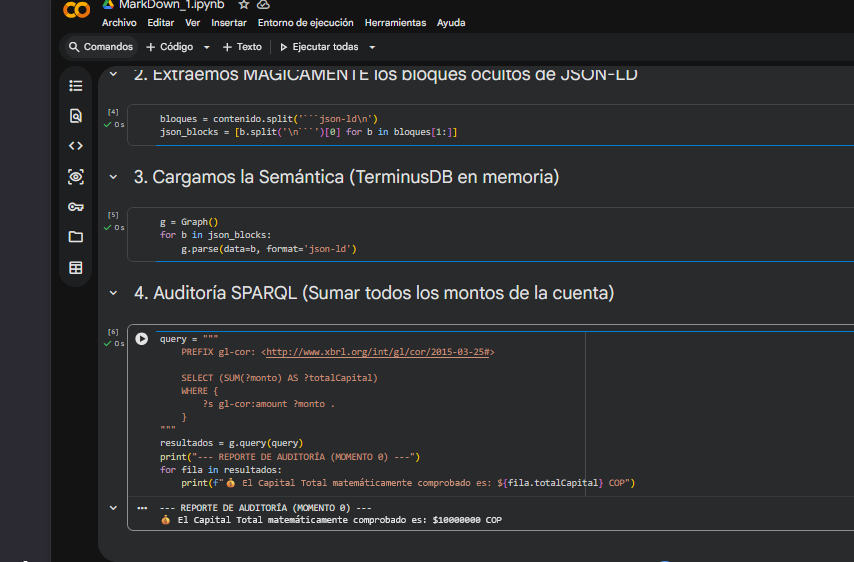
\includegraphics[width=\textwidth]{colab-step2.png}
\caption{SPARQL mathematical verification result: \$10,000,000 COP (Author's Own Work)}
\label{fig:colab2}
\end{figure}

What does that result prove, beyond the arithmetic? It proves that the audit does not need to live where the data was born. An autonomous script---reading nothing but a single Markdown file, with no database connection, no privileged credentials---can reconstruct the full transactional graph and verify its internal consistency. That is what decentralized, continuous auditing looks like in practice.

One nuance worth clarifying here---and it matters operationally---is that TerminusDB exposes two distinct languages for different purposes. QOWL (GraphQL over RDF) is what most practitioners will reach for first: intuitive, declarative, and well-suited to reporting queries. WOQL, the Web Object Query Language, is a different beast entirely. It applies datalog logic directly over the graph, making it the right tool for enforcing the REA transactional rules we described earlier. A WOQL constraint does not merely check a condition---it prevents an inconsistent state from being written in the first place. Updates are atomic, rule-bound, and verifiable. In the A\&AD architecture, WOQL is not an option; it is the enforcement layer.

\hrule
\vspace{1em}
\clearpage

% -----------------------------------------------------------------------
% SECTION 5: CONCLUSION
% -----------------------------------------------------------------------
\section{Conclusion}

A reliance on retrospective reconciliation processes is an outdated habit of the relational database age. As shown by the Accounting and Audit by Design (A\&AD) model, moving verification procedures ``left'' to the moment of data creation is both conceptually sound and technically achievable. By integrating the REA ontology, TerminusDB knowledge graphs, and hybrid DataBooks, organizations can package economic activities into self-contained, self-verifying semantic records.

From the analysis and implementation of this architecture, three key conclusions emerge regarding the benefits of the A\&AD framework:

\begin{enumerate}
\item \textbf{Definitive Eradication of Reconciliation Debt through ``Accounting Shift-Left'':} By capturing and validating the transactional semantics and context at ``Moment~0'' (the origin of the economic event), A\&AD eliminates the need for complex, retrospective reconciliations. Resolving data inconsistency at the point of ingestion removes the reliance on manual spreadsheets for late-stage adjustments, enabling a real-time, friction-free business view.

\item \textbf{Internal Control as a Topological Property of the Graph (SHACL):} Instead of relying on static policy manuals and regulatory limits verified forensically or manually, A\&AD moves governance and compliance rules into hard logical constraints at the database level using SHACL (Shapes Constraint Language). Double-entry balance, authorized signatures, and transaction thresholds become intrinsic, unbreakable properties of the data structure, preventing corrupt records from being written.

\item \textbf{Explainable Governance and Deterministic Auditing for the Agentic AI Era:} A\&AD provides the trust infrastructure required to oversee both human transactions and autonomous decisions executed by AI software agents. Through hybrid DataBooks (Markdown + JSON-LD) and deterministic SPARQL queries on in-memory knowledge graphs, the system enables immediate, high-fidelity, ``zero-shot'' auditing. This substantially reduces the risk of LLM hallucinations during compliance tasks by binding the AI to formal ontological boundaries.
\end{enumerate}

Our future work will focus on extending this proof of concept to handle ongoing operational transactions and deploying real-time SHACL validation guards at the database level, laying the groundwork for automated, model-driven corporate governance. In the financial information supply chain of the AI era, a natural next step will be to integrate A\&AD's origin-point validation with a high-level disclosure mechanics layer---such as the one formalized by the Seattle Method---to produce a fully industrialized digital audit pipeline, where compliance is both designed-in at inception and machine-verifiable at disclosure. Additionally, the full operationalization of A\&AD at scale will require a comprehensive taxonomy of standard business events---as formally defined by bodies such as the FASB and IASB in machine-interpretable form---to complement the framework's genesis-point validation with a structured catalog of the disclosures that each event type must produce. Finally, closing the loop with practical auditing applications, future iterations will focus on automating the generation of traditional audit schedules and working papers directly from the semantic graph, bridging the deterministic proof with the tangible artifacts expected by assurance professionals.

\hrule
\vspace{1em}

\section*{Acknowledgements}

The author wishes to express sincere gratitude to \href{https://www.linkedin.com/in/charleshoffmancpa/}{Charles Hoffman} (CPA, Father of XBRL) for his thoughtful reviews, invaluable feedback, and public endorsement positioning A\&AD as the ``Modern Version of Ricordanze'' (see \href{https://digitalfinancialreporting.blogspot.com/2026/07/modern-version-of-ricordanze.html}{Hoffman, 2026}). Gratitude is also extended to \href{https://www.linkedin.com/in/timathompson/}{Timothy Thompson}, and \href{https://www.linkedin.com/in/deanritz/}{Dean Ritz} (Chief Strategy Officer, DFRNT) for their meticulous feedback on earlier versions of this manuscript. Their collective expertise substantially strengthened the theoretical and technical contributions of this work. Special acknowledgment is due to \href{https://www.linkedin.com/in/hoijnet}{Philippe Höij} (Cofounder \& CEO, \href{https://dfrnt.com}{DFRNT}) for his precise and technically rigorous observations regarding TerminusDB's bitemporal reasoning, the CWA datalog reasoner, and the operational distinction between WOQL and QOWL---contributions that materially elevated the technical depth of Section 3. The author also extends appreciation to the \href{https://www.xbrl.org}{XBRL Consortium} for maintaining the open standards that make this framework possible, and to \href{https://dfrnt.com}{DFRNT} for providing the semantic data platform utilized in the proof of concept.

\vspace{1em}

% -----------------------------------------------------------------------
% BIBLIOGRAPHY
% -----------------------------------------------------------------------
\begin{thebibliography}{99}

\bibitem{actus2018}
ACTUS Financial Research Foundation. (2018). \textit{Algorithmic Contract Types Unified Standards (ACTUS)}. Retrieved from \url{https://www.actusfrf.org/}.

\bibitem{altova2010}
Altova. (2010). \textit{Case Study: Maryland Association of CPAs (MACPA) Integrates Accounting Systems with XBRL GL and Altova MapForce}. Retrieved from \url{https://www.altova.com/documents/macpa_casestudy.pdf}.

\bibitem{bernerslee2001}
Berners-Lee, T., Hendler, J., \& Lassila, O. (2001). The Semantic Web. \textit{Scientific American}, 284(5), 34--43.

\bibitem{cagle2026}
Cagle, K. (2026). \textit{DataBook Pipelines: From Raw Data to Living Knowledge}. The Ontologist. Retrieved from \url{https://ontologist.substack.com/p/databook-pipelines}.

\bibitem{dai2016}
Dai, J., \& Vasarhelyi, M.~A. (2016). Imagineering Audit 4.0. \textit{Journal of Emerging Technologies in Accounting}, 13(1), 1--15.

\bibitem{edmc2020}
EDMC. (2020). \textit{Financial Industry Business Ontology (FIBO)}. Enterprise Data Management Council. Retrieved from \url{https://spec.edmcouncil.org/fibo/}.

\bibitem{fischerpauzenberger2017}
Fischer-Pauzenberger, C., \& Schwaiger, W.~S. (2017). OntoREA: A foundational ontology-based formalization of the REA accounting model. \textit{Journal of Information Systems}, 31(3), 43--69.

\bibitem{fischerpauzenberger2018}
Fischer-Pauzenberger, C., \& Schwaiger, W.~S. (2018). OntoREA\copyright{} Accounting and Finance Model: Hedge Portfolio Representation of Derivatives. In \textit{IFIP Working Conference on The Practice of Enterprise Modeling} (pp.~372--382). Springer, Cham. \url{https://doi.org/10.1007/978-3-030-02302-7_24}

\bibitem{grieves2002}
Grieves, M. (2002). \textit{Conceptual ideal for Product Lifecycle Management (PLM)}. Presented at the Society of Manufacturing Engineers Conference, Troy, Michigan. Retrospectively documented in: Grieves, M., \& Vickers, J. (2017). Digital twin: Mitigating unpredictable, undesirable emergent behavior in complex systems. In \textit{Transdisciplinary Perspectives on Complex Systems} (pp.~85--113). Springer. \url{https://doi.org/10.1007/978-3-319-38756-7_4}

\bibitem{hevner2004}
Hevner, A.~R., March, S.~T., Park, J., \& Ram, S. (2004). Design science in information systems research. \textit{MIS Quarterly}, 28(1), 75--105.

\bibitem{hoffman2025}
Hoffman, C. (2025). \textit{Rethinking Financial Reporting: the Model-driven Financial Statement}. Seattle Method. Retrieved from \url{https://seattlemethod.blogspot.com/}.

\bibitem{mccarthy1982}
McCarthy, W.~E. (1982). The REA accounting model: A generalized framework for accounting systems in a shared data environment. \textit{The Accounting Review}, 57(3), 554--578.

\bibitem{palatucci2009}
Palatucci, M., Pomerleau, D., Hinton, G., \& Mitchell, T. M. (2009). \textit{Zero-shot learning with semantic output codes}. Advances in neural information processing systems, 22.

\bibitem{sorter1969}
Sorter, G.~H. (1969). An ``events'' approach to basic accounting theory. \textit{The Accounting Review}, 44(1), 12--19.

\bibitem{sunder1997}
Sunder, S. (1997). \textit{Theory of Accounting and Control}. South-Western College Publishing.

\bibitem{w3cxbrl}
W3C. (2009a). \textit{XBRL and the Semantic Web}. W3C Interest Group Report. Retrieved from \url{https://www.w3.org/2009/03/xbrl/old-report.html}.

\bibitem{w3cskos}
W3C. (2009b). \textit{SKOS Simple Knowledge Organization System Reference}. W3C Recommendation. Retrieved from \url{https://www.w3.org/TR/skos-reference/}.

\bibitem{mccomb2019}
McComb, D. (2019). \textit{The Data-Centric Revolution: Restoring Sanity to Enterprise Information Systems}. Technics Publications.

\bibitem{dunn2004}
Dunn, C.~L., Cherrington, J.~O., \& Hollander, A.~S. (2004). \textit{Enterprise Information Systems: A Pattern-Based Approach} (3rd ed.). McGraw-Hill. [Foundational reference for REA ontology applied to enterprise information systems.]

\bibitem{gartner2023}
Gartner. (2023). \textit{Digital Twin of an Organization (DTO): How CIOs Can Use Organizational Digital Twins to Enable AI Readiness}. Gartner Research. Retrieved from \url{https://www.gartner.com/en/documents/4228699}.

\end{thebibliography}

\end{document}
